% Options for packages loaded elsewhere
\PassOptionsToPackage{unicode}{hyperref}
\PassOptionsToPackage{hyphens}{url}
\PassOptionsToPackage{dvipsnames,svgnames,x11names}{xcolor}
%
\documentclass[
  10pt,
  dvipsnames]{article}
\usepackage{amsmath,amssymb}
\usepackage{iftex}
\ifPDFTeX
  \usepackage[T1]{fontenc}
  \usepackage[utf8]{inputenc}
  \usepackage{textcomp} % provide euro and other symbols
\else % if luatex or xetex
  \usepackage{unicode-math} % this also loads fontspec
  \defaultfontfeatures{Scale=MatchLowercase}
  \defaultfontfeatures[\rmfamily]{Ligatures=TeX,Scale=1}
\fi
\usepackage{lmodern}
\ifPDFTeX\else
  % xetex/luatex font selection
\fi
% Use upquote if available, for straight quotes in verbatim environments
\IfFileExists{upquote.sty}{\usepackage{upquote}}{}
\IfFileExists{microtype.sty}{% use microtype if available
  \usepackage[]{microtype}
  \UseMicrotypeSet[protrusion]{basicmath} % disable protrusion for tt fonts
}{}
\makeatletter
\@ifundefined{KOMAClassName}{% if non-KOMA class
  \IfFileExists{parskip.sty}{%
    \usepackage{parskip}
  }{% else
    \setlength{\parindent}{0pt}
    \setlength{\parskip}{6pt plus 2pt minus 1pt}}
}{% if KOMA class
  \KOMAoptions{parskip=half}}
\makeatother
\usepackage{xcolor}
\usepackage[a4paper,margin=24mm]{geometry}
\usepackage{longtable,booktabs,array}
\usepackage{calc} % for calculating minipage widths
% Correct order of tables after \paragraph or \subparagraph
\usepackage{etoolbox}
\makeatletter
\patchcmd\longtable{\par}{\if@noskipsec\mbox{}\fi\par}{}{}
\makeatother
% Allow footnotes in longtable head/foot
\IfFileExists{footnotehyper.sty}{\usepackage{footnotehyper}}{\usepackage{footnote}}
\makesavenoteenv{longtable}
\usepackage{graphicx}
\makeatletter
\def\maxwidth{\ifdim\Gin@nat@width>\linewidth\linewidth\else\Gin@nat@width\fi}
\def\maxheight{\ifdim\Gin@nat@height>\textheight\textheight\else\Gin@nat@height\fi}
\makeatother
% Scale images if necessary, so that they will not overflow the page
% margins by default, and it is still possible to overwrite the defaults
% using explicit options in \includegraphics[width, height, ...]{}
\setkeys{Gin}{width=\maxwidth,height=\maxheight,keepaspectratio}
% Set default figure placement to htbp
\makeatletter
\def\fps@figure{htbp}
\makeatother
\setlength{\emergencystretch}{3em} % prevent overfull lines
\providecommand{\tightlist}{%
  \setlength{\itemsep}{0pt}\setlength{\parskip}{0pt}}
\setcounter{secnumdepth}{5}
\ifLuaTeX
\usepackage[bidi=basic]{babel}
\else
\usepackage[bidi=default]{babel}
\fi
\babelprovide[main,import]{korean}
% get rid of language-specific shorthands (see #6817):
\let\LanguageShortHands\languageshorthands
\def\languageshorthands#1{}
\usepackage{fontspec}
\usepackage{needspace}
\microtypesetup{protrusion=false,expansion=false}
\setmainfont[Path=/tmp/vigilode-doc-fonts/,BoldFont=NotoSansKR-Bold.ttf,ItalicFont=NotoSansKR-Regular.ttf,ItalicFeatures={FakeSlant=0.15}]{NotoSansKR-Regular.ttf}
\setsansfont[Path=/tmp/vigilode-doc-fonts/,BoldFont=NotoSansKR-Bold.ttf]{NotoSansKR-Regular.ttf}
\setmonofont{DejaVu Sans Mono}[Scale=0.78]
\XeTeXlinebreaklocale "ko"
\XeTeXlinebreakskip=0pt plus 0.12em
\setlength{\emergencystretch}{3em}
\setlength{\parindent}{0pt}
\setlength{\parskip}{5pt plus 1pt minus 1pt}
\allowdisplaybreaks
\renewcommand{\contentsname}{목차}
\renewcommand{\figurename}{그림}
\renewcommand{\tablename}{표}
\usepackage{fancyhdr}
\pagestyle{fancy}
\fancyhf{}
\fancyhead[L]{\footnotesize VigilODE 수학적 설계}
\fancyhead[R]{\footnotesize 범용 상미분방정식 적분}
\fancyfoot[C]{\thepage}
\setlength{\headheight}{15pt}
\ifLuaTeX
  \usepackage{selnolig}  % disable illegal ligatures
\fi
\IfFileExists{bookmark.sty}{\usepackage{bookmark}}{\usepackage{hyperref}}
\IfFileExists{xurl.sty}{\usepackage{xurl}}{} % add URL line breaks if available
\urlstyle{same}
\hypersetup{
  pdftitle={VigilODE: 범용 상미분방정식 적분기의 수학적 설계},
  pdfauthor={기술 설계 문서},
  pdflang={ko-KR},
  colorlinks=true,
  linkcolor={NavyBlue},
  filecolor={Maroon},
  citecolor={Blue},
  urlcolor={NavyBlue},
  pdfcreator={LaTeX via pandoc}}

\title{VigilODE: 범용 상미분방정식 적분기의 수학적 설계}
\usepackage{etoolbox}
\makeatletter
\providecommand{\subtitle}[1]{% add subtitle to \maketitle
  \apptocmd{\@title}{\par {\large #1 \par}}{}{}
}
\makeatother
\subtitle{명시적 방법과 선형 음시적 방법의 선택, 오차 제어, 실행 계약}
\author{기술 설계 문서}
\date{2026년 10월 24일}

\begin{document}
\maketitle

{
\hypersetup{linkcolor=}
\setcounter{tocdepth}{2}
\tableofcontents
}
\hypertarget{uxcd08uxb85d}{%
\section{초록}\label{uxcd08uxb85d}}

VigilODE의 범용 적분 인터페이스는 초기값 문제의 수학적 성질과 사용자가
허용한 연산을 함께 고려하여 시간 적분 방법을 선택한다. 비강성 문제와
강성이 알려지지 않은 문제에는 우변 평가만을 사용하는 Dormand--Prince
5(4) 방법을 적용한다. 강성 문제에는 도함수 계산이 명시적으로 허용되었을
때 RODAS5P를 적용한다. 전자는 행렬 구성과 선형 풀이를 요구하지 않으며,
후자는 한 시간 간격 안에서 같은 선형 연산자를 재사용하여 비선형 Newton
반복 없이 강성 성분을 처리한다. 두 방법은 성분별 절대 허용오차, 상대
허용오차, 유한성 검사, 시도 횟수 제한, 마지막으로 수락한 상태의
보존이라는 공통 실행 계약을 따른다.

본 문서는 이 두 방법을 중심으로 수학적 정의, 계수, 국소 오차 추정, 보간,
계산량 및 공개 인터페이스의 의미를 기술한다. 특히 도함수를 사용하지 않는
계산과 행렬을 명시적으로 구성하지 않는 계산을 구별하고, 국소 허용오차가
뜻하는 바를 전역 오차와 분리하여 설명한다. 계수의 대수적 성질에서
도출되는 재사용 원리, 선형 풀이의 잔차가 해에 미치는 영향, 가변 시간
간격에 대한 조건부 전역 오차 한계를 증명한다. 이는 특정 응용 분야에
종속되지 않는 상미분방정식 적분기 설계에 대한 기술이다.

\hypertarget{uxbb38uxc81c-uxc124uxc815uxacfc-uxc124uxacc4uxc758-uxb3d9uxae30}{%
\section{문제 설정과 설계의
동기}\label{uxbb38uxc81c-uxc124uxc815uxacfc-uxc124uxacc4uxc758-uxb3d9uxae30}}

\hypertarget{uxc801uxbd84-uxb300uxc0c1uxacfc-uxc804uxc81c}{%
\subsection{적분 대상과
전제}\label{uxc801uxbd84-uxb300uxc0c1uxacfc-uxc804uxc81c}}

대상은 유한한 전진 시간 구간에서 정의된 초기값 문제

\[
 y'(t)=f(t,y(t)),\qquad y(t_0)=y_0\in\mathbb R^n,
 \qquad t_0\le t\le T
 \tag{1}
\]

이다. 상태와 시간은 IEEE 754 배정밀도 실수로 표현한다. 일반 인터페이스의
질량행렬은 항등행렬이다. 콜백은 동일한 시간과 상태에 대해 동일한 우변을
반환해야 하며, 수락되지 않은 시도 중에 외부의 모델 매개변수를 바꾸어서는
안 된다. 상태 차원, 성분의 의미 및 허용오차의 단위도 한 적분 실행 동안
고정된다. 이 전제는 수학적 방법뿐 아니라 거절한 시간 간격의 재시도와
저장된 우변 값의 재사용에 필요하다.

오차 차수에 대한 명제에는 추가 가정을 둔다. 정확해를 포함하는 근방에서
\(f\)가 필요한 차수까지 미분 가능하고, 해와 관련 도함수가 유계이며, 시간
간격이 해당 방법의 안정성과 오차 전개가 유효한 범위에 있어야 한다.
불연속 우변, 구간별 모델 전환 또는 특이점을 포함하는 문제를 매끄러운
문제의 차수 정리로 해석하지 않는다. 알려진 불연속점은 적분 구간을 나누는
경계로 처리할 수 있다.

\hypertarget{uxd558uxb098uxc758-uxace0uxbe44uxc6a9-uxbc29uxbc95uxc73cuxb85c-uxbaa8uxb4e0-uxbb38uxc81cuxb97c-uxcc98uxb9acuxd558uxc9c0-uxc54auxb294-uxc774uxc720}{%
\subsection{하나의 고비용 방법으로 모든 문제를 처리하지 않는
이유}\label{uxd558uxb098uxc758-uxace0uxbe44uxc6a9-uxbc29uxbc95uxc73cuxb85c-uxbaa8uxb4e0-uxbb38uxc81cuxb97c-uxcc98uxb9acuxd558uxc9c0-uxc54auxb294-uxc774uxc720}}

강성 문제에서는 해가 천천히 변하더라도 빠르게 감쇠하는 성분 때문에
명시적 방법의 안정성 제한이 엄격해질 수 있다. 반대로 이러한 제한이 없는
작은 문제에서 매 시간 간격마다 Jacobian과 LU 분해를 구성하면 우변을
평가하는 비용보다 부수적인 연산이 더 커질 수 있다. 따라서 범용성은 모든
문제에 동일한 대수 연산을 적용하는 것으로 정의하지 않는다. 서로 다른
계산 구조를 가진 두 방법을 공통의 입력과 실패 계약으로 제공하는 데서
출발한다.

고주파 진동 역시 강성과 구분한다. \(y'=i\omega y\)의 진폭은 일정하지만,
수치해의 위상은 작은 간격별 오차를 장시간 누적할 수 있다. 왼쪽
반평면에서의 안정성은 이러한 위상 정확도를 대신하지 않는다. 따라서
문제의 강성 선언은 방법 선택에 필요한 정보이고, 실제로 필요한 시간
해상도는 허용오차와 관측량의 정확도 요구에 의해 정해진다.

\hypertarget{uxbc29uxbc95-uxc120uxd0dduxacfc-uxacf5uxac1c-uxc0acuxc591}{%
\section{방법 선택과 공개
사양}\label{uxbc29uxbc95-uxc120uxd0dduxacfc-uxacf5uxac1c-uxc0acuxc591}}

\hypertarget{uxc120uxc5b8uxc5d0-uxb530uxb978-uxc120uxd0dd}{%
\subsection{선언에 따른
선택}\label{uxc120uxc5b8uxc5d0-uxb530uxb978-uxc120uxd0dd}}

일반 진입점은 \texttt{GeneralOde::solve}이다.
\texttt{GeneralOdePolicy}는 문제 유형을 \texttt{ProblemRegime}으로
지정하고, \texttt{derivatives:\ DerivativeFallback}으로 도함수 계산 허용
여부를, \texttt{max\_dense\_dimension}으로 조밀 행렬 사용의 자원 한계를
명시한다. 기본 선택에서 강성이 알려지지 않은 문제는 명시적 방법으로
시작한다. 실행 중 수집한 경험적 수치만으로 도함수 계산을 새로 허용하거나
다른 방법으로 몰래 바꾸지 않는다.

\Needspace{8\baselineskip}
\begin{longtable}[]{@{}
  >{\raggedright\arraybackslash}p{(\columnwidth - 6\tabcolsep) * \real{0.2500}}
  >{\raggedright\arraybackslash}p{(\columnwidth - 6\tabcolsep) * \real{0.2500}}
  >{\raggedright\arraybackslash}p{(\columnwidth - 6\tabcolsep) * \real{0.2500}}
  >{\raggedright\arraybackslash}p{(\columnwidth - 6\tabcolsep) * \real{0.2500}}@{}}
\toprule\noalign{}
\begin{minipage}[b]{\linewidth}\raggedright
입력 조건
\end{minipage} & \begin{minipage}[b]{\linewidth}\raggedright
선택 방법
\end{minipage} & \begin{minipage}[b]{\linewidth}\raggedright
핵심 연산
\end{minipage} & \begin{minipage}[b]{\linewidth}\raggedright
사용자에게 요구하는 정보
\end{minipage} \\
\midrule\noalign{}
\endhead
\bottomrule\noalign{}
\endlastfoot
\texttt{Unknown} & DOPRI5 & 우변 평가와 벡터 결합 & \(f(t,y)\) \\
\texttt{Nonstiff} & DOPRI5 & 우변 평가와 벡터 결합 & \(f(t,y)\) \\
\texttt{Stiff}, 도함수 계산 허용 & RODAS5P & 우변, Jacobian 정보, 선형
풀이 & 제공 도함수 또는 허용된 수치 미분 \\
\texttt{Stiff}, 도함수 계산 불허 & 실행 전 오류 & 없음 & 허용 정책 변경
또는 다른 방법의 직접 선택 \\
\end{longtable}

기본 조밀 행렬 차원 한계는 \(n=64\)이다. 이는 수학적 적용 한계가 아니라
메모리와 분해 비용을 통제하는 구성값이다. 사용자는 해당 비용을 알고
한계를 변경할 수 있다. 대역 구조가 주어진 경우에는 그 구조를 이용하는
경로를 선택한다. 조밀 Jacobian 콜백에 대역 선언을 덧붙인 경우에는 여전히
조밀 배열을 구성하므로 차원 한계가 적용된다. 압축된 대역 콜백이나 대역
유한차분만 이 한계에서 제외된다. Jacobian--벡터 곱을 이용하는 경로는
\texttt{allow\_matrix\_free=true}를 요구하며 기본값은
\texttt{false}이다. 알려지지 않은 강성에 대해 명시적 방법을 선택한다는
것은 그 문제에서 빠른 완료를 보장한다는 뜻이 아니다. 시간 간격 축소나
시도 횟수 소진은 진단 가능한 결과로 반환된다.

\texttt{DerivativeFallback::Forbidden}은 도함수 계산을 금지하는
기본값이다. \texttt{ProvidedOnly}는 제공된 Jacobian 또는 JVP와, 비자율
문제에서 제공된 시간 편미분을 요구한다. 자율 문제는
\texttt{autonomous()}로 시간 편미분이 0임을 선언할 수 있다.
\texttt{AllowFiniteDifference}는 빠진 도함수를 수치 미분으로 계산하도록
허용한다. \texttt{GeneralOde::select}는 우변을 호출하지 않고 이 기능과
권한의 조합을 확인한다. 시간 구간, 초기 상태 및 허용오차의 수치적
유효성은 \texttt{solve}에서 검사한다.

\hypertarget{uxc9c0uxc6d0-uxbc94uxc704}{%
\subsection{지원 범위}\label{uxc9c0uxc6d0-uxbc94uxc704}}

일반 인터페이스는 항등 질량행렬의 ODE와 고정 차원 상태를 다루며 끝점
결과를 반환한다. \texttt{dense\_output=true}인 요청은 거부하고, 연속
출력은 방법별 직접 인터페이스에서 요청한다. 사건 함수에 따른 근 위치
탐색, 사건 직후 상태 변경, 질량행렬 및 대수 제약은 이 인터페이스의
계약에 포함되지 않는다. 지원하지 않는 조합은 우변을 호출하기 전에
거부한다. 각 방법의 직접 인터페이스에서 제공하는 출력 기능은 아래와
같다. 이 직접 인터페이스의 출력 확장은 자동 방법 선택 기능과 구별한다.

\begin{longtable}[]{@{}
  >{\raggedright\arraybackslash}p{(\columnwidth - 4\tabcolsep) * \real{0.3333}}
  >{\raggedright\arraybackslash}p{(\columnwidth - 4\tabcolsep) * \real{0.3333}}
  >{\raggedright\arraybackslash}p{(\columnwidth - 4\tabcolsep) * \real{0.3333}}@{}}
\toprule\noalign{}
\begin{minipage}[b]{\linewidth}\raggedright
기능
\end{minipage} & \begin{minipage}[b]{\linewidth}\raggedright
DOPRI5
\end{minipage} & \begin{minipage}[b]{\linewidth}\raggedright
RODAS5P
\end{minipage} \\
\midrule\noalign{}
\endhead
\bottomrule\noalign{}
\endlastfoot
끝점 적분 & 지원 & 지원 \\
성분별 절대 허용오차 & 지원 & 선택한 직접 선형 풀이 경로에서 지원 \\
지정 시각에 실제 시간 간격 종료 & \texttt{solve\_observed} & 공개
인터페이스는 구간 양 끝점만 제공 \\
지정 시각의 연속 보간 표본 & \texttt{solve\_dense\_observed} & 연속 출력
경로 \\
실행 후 임의 시각의 보간 객체 & 일반 DOPRI5 진입점에서는 제공하지 않음 &
조밀 또는 대역 연속 출력 경로 \\
수락한 상태에서 일시 중지와 재개 & \texttt{Dopri5::with\_session} & 본
문서의 일반 인터페이스에는 포함하지 않음 \\
우변만으로 수행 & 예 & 아니오 \\
Newton 비선형 반복 & 없음 & 없음 \\
\end{longtable}

\texttt{Options::dense\_output}은 실행 뒤에도 보관할 연속 출력 객체를
요청하는 설정이다. 이 설정을 DOPRI5에 주는 것과
\texttt{solve\_dense\_observed}로 표본만 요청하는 것은 서로 다른
계약이다. 전자는 거부되고, 후자는 지원된다. RODAS5P의 Jacobian--벡터 곱
경로는 끝점 출력에 한정되며, 성분별 절대 허용오차도, 연속 출력도 해당
경로에서 지원하지 않는다. 스칼라 절대 허용오차를 사용한 끝점 출력만
지원한다.

\hypertarget{uxba85uxc2dcuxc801-dormandprince-54-uxbc29uxbc95}{%
\section{명시적 Dormand--Prince 5(4)
방법}\label{uxba85uxc2dcuxc801-dormandprince-54-uxbc29uxbc95}}

\hypertarget{uxb2e8uxacc4uxc2dduxacfc-uxacc4uxc218}{%
\subsection{단계식과 계수}\label{uxb2e8uxacc4uxc2dduxacfc-uxacc4uxc218}}

Dormand--Prince 방법은 같은 우변 평가로 5차 근사와 4차 근사를 구성하는
내장 Runge--Kutta 쌍이다 {[}1{]}. 시간 간격 \(h>0\)에 대하여 일곱 단계의
도함수 값을

\[
 k_i=f\!\left(t_n+c_i h,\;y_n+h\sum_{j<i}a_{ij}k_j\right),
 \qquad i=1,\ldots,7
 \tag{2}
\]

로 계산한다. 수락 후보와 내장 오차 벡터는

\[
 y_{n+1}=y_n+h\sum_{i=1}^7 b_i k_i,\qquad
 e_n=h\sum_{i=1}^7(b_i-\widehat b_i)k_i
 \tag{3}
\]

이다. 구현은 두 끝점 벡터를 계산한 뒤 빼는 대신 마지막 식의 가중합을
직접 계산한다. 이 선택은 큰 상태값끼리의 불필요한 상쇄를 피한다.

\begin{equation}\resizebox{0.98\textwidth}{!}{$\renewcommand{\arraystretch}{1.25}
\begin{array}{c|rrrrrrr}
0&0&0&0&0&0&0&0\\
1/5&1/5&0&0&0&0&0&0\\
3/10&3/40&9/40&0&0&0&0&0\\
4/5&44/45&-56/15&32/9&0&0&0&0\\
8/9&19372/6561&-25360/2187&64448/6561&-212/729&0&0&0\\
1&9017/3168&-355/33&46732/5247&49/176&-5103/18656&0&0\\
1&35/384&0&500/1113&125/192&-2187/6784&11/84&0\\\hline
b&35/384&0&500/1113&125/192&-2187/6784&11/84&0\\
\widehat b&5179/57600&0&7571/16695&393/640&-92097/339200&187/2100&1/40
\end{array}$}\tag{4}\end{equation}

표의 첫 열은 \(c_i\)이며 나머지 열은 \(a_{ij}\)이다. \(b\)를 사용한
끝점의 국소 절단오차는 매끄러운 문제에서 \(O(h^6)\), 내장 차이는
일반적으로 \(O(h^5)\)이다. 따라서 간격 제어기의 지수는 \(1/5\)이다. 끝점
공식이 5차라는 이유로 내장 차이에 \(1/6\)을 적용하지 않는다.

\hypertarget{uxcc28uxc218-uxc870uxac74uxc758-uxb300uxc218uxc801-uxd655uxc778}{%
\subsection{차수 조건의 대수적
확인}\label{uxcc28uxc218-uxc870uxac74uxc758-uxb300uxc218uxc801-uxd655uxc778}}

\textbf{명제 1.} 식 (4)의 유리수 계수는 일반 비선형 ODE에 대한 명시적
Runge--Kutta 방법의 5차 조건을 만족하며, \(\widehat b\)는 4차 조건을
만족한다.

\textbf{증명.} 뿌리 나무 \(\tau\)의 꼭짓점 수를 \(|\tau|\)라 하고,

\[
 d(\bullet)=1,\qquad
 d([\tau_1,\ldots,\tau_m])=|\tau|\prod_{q=1}^m d(\tau_q)
 \tag{5}
\]

를 정의한다. 단계별 기본 가중치는

\[
 \Phi_i(\bullet)=1,\qquad
 \Phi_i([\tau_1,\ldots,\tau_m])
 =\prod_{q=1}^m\left(\sum_j a_{ij}\Phi_j(\tau_q)\right)
 \tag{6}
\]

이다. 미분의 연쇄법칙으로 정확한 흐름과 식 (2)를 전개하면, 같은 나무에
대응하는 기본 미분항의 계수가 일치할 필요충분조건은
\(b^T\Phi(\tau)=1/d(\tau)\)이다. 비동차 시간 의존성은 \(t'=1\)을 추가한
자율계로 옮긴다. 이때 필요한 \(c=A\mathbf1\)도 식 (4)에서 성립한다.

차수 \(1,2,3,4,5\)에서 서로 다른 나무의 수는 각각 \(1,1,2,4,9\)개이다.
예를 들어 1차 조건은 \(b^T\mathbf1=1\), 2차 조건은 \(b^Tc=1/2\), 3차
조건은 \(b^Tc^2=1/3\) 및 \(b^TAc=1/6\)이다. 식 (5)와 (6)에 식 (4)의
유리수를 대입하면 5차까지 17개 등식의 잔차가 모두 정확히 0이다. 같은
계산에서 \(\widehat b\)는 4차까지 8개 등식을 만족한다. 나머지 Taylor
항은 필요한 도함수가 유계인 근방에서 각각 \(O(h^6)\)와 \(O(h^5)\)이므로
결론을 얻는다. 실제 기계 연산에서는 유리수의 배정밀도 표현과 반올림
오차가 추가된다. \(\square\)

\hypertarget{uxb9c8uxc9c0uxb9c9-uxb2e8uxacc4uxc758-uxc7acuxc0acuxc6a9}{%
\subsection{마지막 단계의
재사용}\label{uxb9c8uxc9c0uxb9c9-uxb2e8uxacc4uxc758-uxc7acuxc0acuxc6a9}}

\textbf{명제 2.} 수락한 단계의 \(k_7\)은 다음 단계의 \(k_1\)으로
재사용할 수 있다. 단, 우변 함수와 상태의 의미가 바뀌지 않아야 한다.

\textbf{증명.} 식 (4)에서 \(c_7=1\), \(a_{7j}=b_j\)이고 \(b_7=0\)이다.
따라서

\[
 k_7=f\!\left(t_n+h,y_n+h\sum_jb_jk_j\right)
     =f(t_{n+1},y_{n+1}).
 \tag{7}
\]

이는 다음 시간 간격의 첫 우변 값과 같다. 거절한 시도에서는
\((t_n,y_n)\)가 유지되므로 기존의 첫 우변을 재사용할 수 있지만, 거절한
후보 끝점의 \(k_7\)을 재사용해서는 안 된다. \(\square\)

첫 시도에는 일곱 번의 우변 평가가 필요하고, 정상적인 연속 수락에서는
이후 한 시도당 여섯 번의 새 평가가 필요하다. 이 절감은 추가적인 근사에
의한 것이 아니라 계수 항등식에 의한 것이다. 저장된 도함수는 모델, 상태
또는 설정의 유효성이 바뀌면 폐기해야 한다.

\hypertarget{uxc548uxc815uxc131uxacfc-uxc9c4uxb3d9-uxc624uxcc28}{%
\subsection{안정성과 진동
오차}\label{uxc548uxc815uxc131uxacfc-uxc9c4uxb3d9-uxc624uxcc28}}

선형 시험방정식 \(y'=\lambda y\)에 식 (2)를 대입하고 \(z=h\lambda\)라
하면

\[
 y_{n+1}=R(z)y_n,\qquad
 R(z)=\sum_{j=0}^{5}\frac{z^j}{j!}+\frac{z^6}{600}.
 \tag{8}
\]

이는 유한 다항식이므로 모든 왼쪽 반평면에서 안정한 방법은 아니다. 음의
실축에서 큰 \(|z|\)를 갖는 강성 성분에는 시간 간격 제한이 생긴다. 반면
충분히 작은 진동 간격 \(z=i\theta\)에서는 정확한 증폭인자
\(e^{i\theta}\)와 가깝다. 진폭 오차는 \(|R(i\theta)|-1\), 한 간격의 위상
오차는 \(\arg R(i\theta)-\theta\)로 구분하여 해석한다.

\textbf{명제 3.} \(y'=i\omega y\), \(|y_0|=1\)에 가변 간격 \(h_j>0\)를
적용하고, \(\sum_jh_j=T\) 및 \(|\omega|h_j\le0.9\)라 하자. 정확한
산술에서

\[
 \left|y_N-e^{i\omega T}y_0\right|
 \le T|\omega|^6 h_{\max}^5
 \left(\frac1{3600}+\frac{0.9e^{0.9}}{5040}\right).
 \tag{9}
\]

\textbf{증명.} 다항식 (8)을 전개하면

\[
 |R(i\theta)|^2-1
 =\frac{\theta^6}{360000}
 \left(\theta^6-25\theta^4+225\theta^2-200\right).
 \tag{10}
\]

\(x=\theta^2\in[0,0.81]\)에서 괄호는 \(x^3-25x^2+225x-200\le0\)이다.
따라서 \(|R(i\theta)|\le1\)이다. Taylor 나머지를 이용하면

\[
 |R(i\theta)-e^{i\theta}|
 \le\frac{|\theta|^6}{3600}
   +\frac{|\theta|^7e^{|\theta|}}{7!}.
 \tag{11}
\]

수치 증폭인자들의 곱과 정확한 증폭인자들의 곱의 차이를 망원합으로 쓰면,
다른 인자들의 절댓값이 1 이하이므로 전체 차이는 식 (11)의 합 이하이다.
마지막으로 \(\sum_j h_j^6\le h_{\max}^5T\)를 적용한다. \(\square\)

이 명제는 선형 정규 진동에 대한 구체적인 충분조건이다. 일반적인 비정규
행렬, 시간 의존 주파수 또는 비선형 진동에 같은 상수를 적용하지 않는다.
또한 간격별 국소 오차 검사를 통과했다는 사실만으로 식 (9)의 가정인 최대
위상 간격이 자동으로 주어지는 것은 아니다.

\begin{figure}
\centering
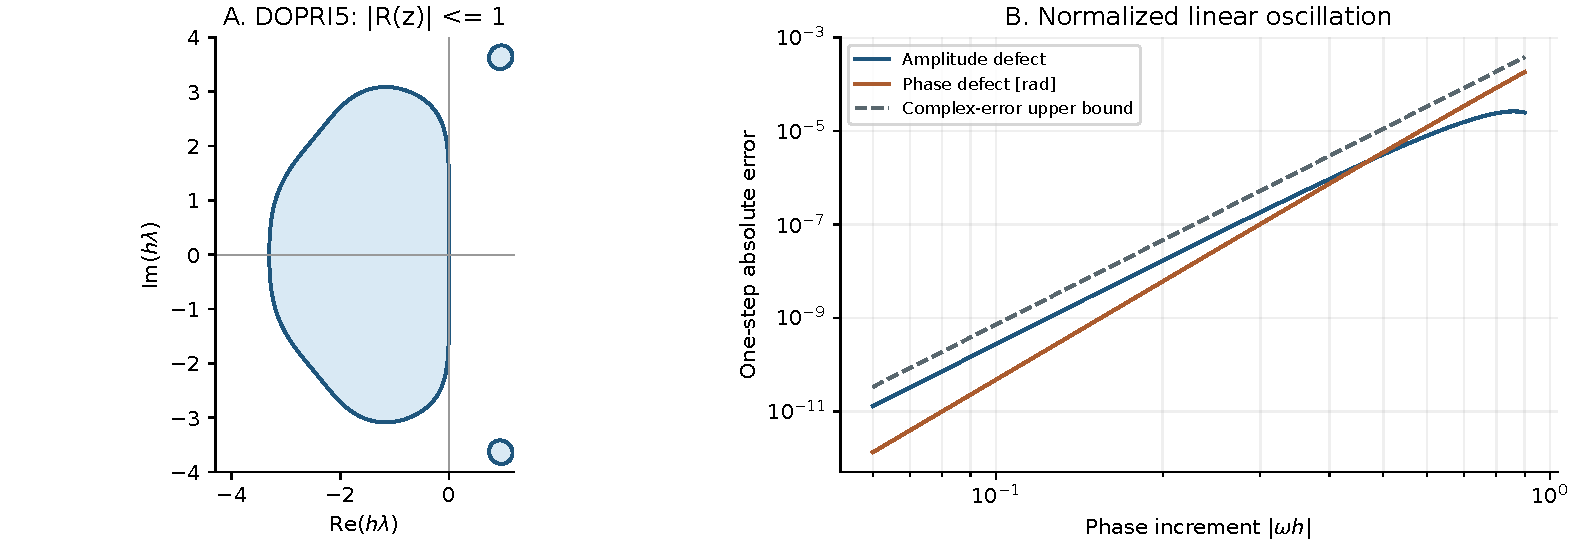
\includegraphics{figures/dopri5_stability.pdf}
\caption{DOPRI5의 안정성 영역과 선형 진동의 한 간격 오차. 왼쪽은 식
(8)의 절대 안정성 영역이다. 오른쪽은 정확한 증폭인자와 비교한 진폭·위상
차이 및 식 (11)의 상한이다. 계산 시간 측정값이 아니라 계수 다항식에서
계산한 양이다.}
\end{figure}

\hypertarget{uxac15uxc131-uxbb38uxc81cuxb97c-uxc704uxd55c-rodas5p}{%
\section{강성 문제를 위한
RODAS5P}\label{uxac15uxc131-uxbb38uxc81cuxb97c-uxc704uxd55c-rodas5p}}

\hypertarget{uxd55c-uxc2dcuxac04-uxac04uxaca9uxc5d0uxc11c-uxd558uxb098uxc758-uxc120uxd615-uxc5f0uxc0b0uxc790uxb97c-uxacf5uxc720uxd558uxb294-uxad6cuxc870}{%
\subsection{한 시간 간격에서 하나의 선형 연산자를 공유하는
구조}\label{uxd55c-uxc2dcuxac04-uxac04uxaca9uxc5d0uxc11c-uxd558uxb098uxc758-uxc120uxd615-uxc5f0uxc0b0uxc790uxb97c-uxacf5uxc720uxd558uxb294-uxad6cuxc870}}

RODAS5P는 5(4)차 Rosenbrock 방법이며, 본 구현의 계수 집합은 여덟 단계를
갖는다. Steinebach의 구성은 강성 문제에서의 차수 저하를 완화하는 조건과
4차 연속 출력 계수를 함께 고려한다 {[}2{]}. 여기서는 구현에 직접
대응하는 변환된 단계 변수 \(u_i\)를 사용한다. \(J_n\)은 \(f_y(t_n,y_n)\)
또는 허용된 근사이고 \(f_{t,n}\)은 상태를 고정한 시간 편미분이다. 다음을
정의한다.

\[
 \gamma=0.21193756319429014,\qquad
 W_n=\frac{I}{h\gamma}-J_n.
 \tag{12}
\]

계수 행렬 \(A=(a_{ij})\)와 \(C=(C_{ij})\)는 엄밀히 하삼각이다. 시간
절점은 \(c_i\), 출력 가중치는 \(b_i^{\rm u}\)이다. 단계식은

\[
\begin{split}
 Y_i&=y_n+\sum_{j<i}a_{ij}u_j,\\
 W_nu_i&=f(t_n+c_i h,Y_i)
       +\frac1h\sum_{j<i}C_{ij}u_j
       +h g_i f_{t,n},\qquad i=1,\ldots,8,\\
 y_{n+1}&=y_n+\sum_{i=1}^8 b_i^{\rm u}u_i,
 \qquad e_n=u_8.
\end{split}
\tag{13}
\]

이다. 여기서

\[
 \Gamma=\left(\gamma^{-1}I_8-C\right)^{-1},\qquad
 g=\Gamma\mathbf1.
 \tag{14}
\]

이다. 조밀 및 대역 직접 풀이에서는 한 시도마다 \(W_n\)을 한 번 분해하고,
여덟 우변에 대해 전후진 대입을 수행한다. 단계별 비선형 방정식을 Newton
반복으로 풀지 않는다. 다만 선형계와 Jacobian 정보는 실제 계산의
일부이다.

\hypertarget{uxbcc0uxc218-uxbcc0uxd658uxc758-uxb3d9uxb4f1uxc131uxacfc-uxc5f0uxc0b0-uxc808uxac10}{%
\subsection{변수 변환의 동등성과 연산
절감}\label{uxbcc0uxc218-uxbcc0uxd658uxc758-uxb3d9uxb4f1uxc131uxacfc-uxc5f0uxc0b0-uxc808uxac10}}

\textbf{명제 4.} 식 (13)은 \(u=\Gamma K\)와 \(\alpha=A\Gamma\)를
사용하는 Rosenbrock 단계식

\[
 (I-h\gamma J_n)K_i
 =h f\!\left(t_n+c_i h,y_n+\sum_{j<i}\alpha_{ij}K_j\right)
 +hJ_n\sum_{j<i}\Gamma_{ij}K_j+h^2g_if_{t,n}
 \tag{15}
\]

과 정확한 산술에서 동등하다.

\textbf{증명.} 여덟 단계의 벡터를 묶어 식 (15)를 쓰면

\[
 \frac1hK-J_n\Gamma K=F+hgf_{t,n}.
 \tag{16}
\]

\(u=\Gamma K\)를 대입하고 \(\Gamma^{-1}=\gamma^{-1}I_8-C\)를 사용하면

\[
 \left(\frac{I}{h\gamma}-J_n\right)u_i
 =F_i+\frac1h\sum_{j<i}C_{ij}u_j+hg_if_{t,n}.
 \tag{17}
\]

또한 \(A u=A\Gamma K=\alpha K\)이므로 단계의 우변 평가점도 같다.
\(\Gamma\)는 대각성분이 \(\gamma\ne0\)인 하삼각행렬이므로 변환은
가역이다. \(\square\)

식 (13)은 식 (15)의 \(J_n\sum_{j<i}\Gamma_{ij}K_j\)를 직접 계산할 필요가
없다. 따라서 동일한 방법을 적용하면서 단계 우변 구성에 필요한
Jacobian--벡터 곱을 제거한다. 이 항등식이 단계 사이의 인과적 의존성을
없애는 것은 아니다. \(Y_i\)는 이전 \(u_j\)를 사용하므로 본 구현의 한
궤적에 대한 여덟 단계는 순서대로 평가된다.

실제 계수는 배정밀도로 파싱한 십진 상수이다. 저자의 수학적 방법이 갖는
형식적 차수와 특정 계수 파일을 유한 정밀도로 실행할 때의 오차를
구분한다. 이 문서의 변수 변환 증명은 주어진 계수에 대한 항등식을
보장한다. 임의의 근사 Jacobian이나 부정확한 선형 풀이에서도 5차가
유지된다는 주장은 이 증명에 포함되지 않는다.

\hypertarget{uxb3c4uxd568uxc218uxc640-uxc120uxd615-uxb300uxc218uxc758-uxc758uxbbf8}{%
\subsection{도함수와 선형 대수의
의미}\label{uxb3c4uxd568uxc218uxc640-uxc120uxd615-uxb300uxc218uxc758-uxc758uxbbf8}}

제공된 조밀 또는 대역 Jacobian은 사용자가 계산한 \(f_y\)를 반환한다.
도함수가 제공되지 않고 수치 미분이 허용된 경우, 조밀 전진차분은

\[
 \begin{aligned}
 (J_n)_{ij}&\approx
 \frac{f_i(t_n,y_n+\delta_j e_j)-f_i(t_n,y_n)}{\delta_j},\\
 \delta_j&=\operatorname{fl}(y_{n,j}+\eta_j)-y_{n,j},\qquad
 \eta_j=\sqrt{\varepsilon_{\rm mach}}\max(1,|y_{n,j}|).
 \end{aligned}
 \tag{18}
\]

를 사용한다. 양의 방향 이동이 유한 범위를 벗어나면 음의 방향 차분을
사용한다. 분모는 수학적으로 요청한 이동량이 아니라 실제 표현된
이동량이다. 한 조밀 Jacobian 구성에는 \(n+1\)회의 우변 평가가 필요하다.
유한차분은 사용자가 해석적 도함수를 제공할 필요를 줄이지만, 도함수를
전혀 사용하지 않는 알고리즘은 아니다.

하부 및 상부 대역폭을 \(\ell,u\)라 하면, 서로 \(w=\ell+u+1\)열씩 떨어진
열들의 비영 행 범위가 겹치지 않는다. 이 구조가 모든 관련 상태에서
정확하다는 전제 아래 같은 묶음의 열을 한 번에 섭동할 수 있다. 한
Jacobian에 필요한 우변 평가 수는 \(1+\min(w,n)\)회로 줄어든다. 대역을
잘못 선언하면 누락된 결합을 수치적으로 복구할 수 없으므로, 대역 선언은
사용자의 수학적 계약이다.

비자율 문제에서 \(f_t\)를 제공하지 않으면 상태를 고정한 중심차분

\[
 f_{t,n}\approx\frac{f(t_n+\epsilon_t,y_n)-f(t_n-\epsilon_t,y_n)}{2\epsilon_t},
 \qquad \epsilon_t=\sqrt{\varepsilon_{\rm mach}}\max(1,|t_n|)
 \tag{19}
\]

을 사용한다. 이는 두 번의 우변 평가를 더 요구하며, 시간 정의역 바깥의
평가가 허용되지 않는 문제에서는 사용자가 시간 편미분을 제공해야 한다.
\texttt{autonomous()}는 실제로 \(f_t=0\)인 문제에서만 지정한다. 잘못된
자율성 선언은 단계식 자체를 바꾼다.

Jacobian--벡터 곱 \(v\mapsto J_nv\)를 제공하면 전체 Jacobian을 저장하지
않는 선형 반복 풀이가 가능하다. 이 경로는 행렬을 명시적으로 구성하지
않는다는 의미에서 matrix-free이며, 도함수의 작용을 사용한다는 사실은
변하지 않는다. 자동미분은 사용자가 제공하는 도함수 작용의 계산 방식일 수
있으나, 일반 선택기가 자동으로 실행하는 기본 연산이 아니다. 선택된 JVP
경로는 재시작 길이 40, 전체 Arnoldi 반복 상한 200, 선형 상대 허용오차
\(10^{-10}\), 설정된 절대 허용오차 \(10^{-14}\)인 GMRES를 사용한다.
실제로 푸는 \((I-h\gamma J_n)u=b_u\) 좌표에서는 절대 잔차 예산을
\(|\gamma|10^{-14}\)로 변환하고 보수적으로 아래 방향 반올림한다. 상대
잔차의 척도는 이 좌표의 우변 \(b_u\)의 2-노름이다. 실제 종료 조건은
\(\|r_u\|_2\le\max(\operatorname{atol}_u,10^{-10}\|b_u\|_2)\)이다. 초기
선형해는 0이며 전처리기는 사용하지 않는다. 일반 선택 인터페이스는 별도의
전처리기를 주입하는 기능을 노출하지 않는다.

\hypertarget{uxc120uxd615-uxc794uxcc28uxc640-uxc0c1uxd0dc-uxc624uxcc28}{%
\subsection{선형 잔차와 상태
오차}\label{uxc120uxd615-uxc794uxcc28uxc640-uxc0c1uxd0dc-uxc624uxcc28}}

\textbf{명제 5.} 가역 행렬 \(W\)에 대한 정확해 \(u\)와 근사해
\(\widetilde u\)가 \(Wu=b\), \(r=b-W\widetilde u\)를 만족하면

\[
 \|u-\widetilde u\|\le\|W^{-1}\|\,\|r\|.
 \tag{20}
\]

\textbf{증명.} \(W(u-\widetilde u)=r\)에 \(W^{-1}\)을 곱하고 일관된
노름의 부곱셈성을 적용한다. \(\square\)

작은 잔차만으로 작은 상태 오차가 보장되지는 않는다. 식 (20)에는
역연산자의 증폭이 함께 들어간다. 단계 간 오차 전파도 다음과 같이
정량화할 수 있다. 동일한 \(W\), \(y_n\), \(f_t\)를 쓰고, 각 단계 우변의
상태 Lipschitz 상수를 \(L_i\)라 하자. 여기서 \(r_i\)는 근사된 이전
단계들로 구성한 실제 선형 우변
\(b_i(\widetilde u_1,\ldots,\widetilde u_{i-1})\)에 대한 잔차, 즉
\(r_i=b_i(\widetilde u_1,\ldots,\widetilde u_{i-1})-W\widetilde u_i\)이다.
\(d_i=\|u_i-\widetilde u_i\|\), \(\kappa=\|W^{-1}\|\)이면

\[
 d_i\le\kappa\|r_i\|+
 \sum_{j<i}\kappa\left(L_i|a_{ij}|+\frac{|C_{ij}|}{h}\right)d_j.
 \tag{21}
\]

\textbf{증명.} 두 단계식의 차이를 취하고, 비선형 우변의 차이에 Lipschitz
부등식을 적용한 뒤 식 (20)을 사용한다.
\(q_{ij}=\kappa(L_i|a_{ij}|+|C_{ij}|/h)\)를 원소로 하는 엄밀히
하삼각행렬 \(Q\)를 정의하면 \(Q^8=0\)이다. 따라서

\[
 d\le(I-Q)^{-1}\kappa\rho
   =\left(I+Q+\cdots+Q^7\right)\kappa\rho,
 \quad \rho_i=\|r_i\|,
 \tag{22}
\]

이며 끝점 오차는 \(|b^{\rm u}|^Td\) 이하이다. \(\square\)

이 결과는 선형 풀이 허용오차를 상태 허용오차와 연결하는 충분조건이다.
현재 모든 직접 풀이에서 이 역노름을 계산하여 인증한다는 뜻은 아니다.
Jacobian 근사 오차, 우변 계산 오차 및 반올림은 별도 섭동으로 추가된다.
따라서 선형 반복 횟수만으로 시간 적분 정확도를 판정하지 않는다.

\hypertarget{uxc801uxc751uxd615-uxc2dcuxac04-uxac04uxaca9uxacfc-uxc815uxd655uxb3c4-uxacc4uxc57d}{%
\section{적응형 시간 간격과 정확도
계약}\label{uxc801uxc751uxd615-uxc2dcuxac04-uxac04uxaca9uxacfc-uxc815uxd655uxb3c4-uxacc4uxc57d}}

\hypertarget{uxc131uxbd84uxbcc4-uxc624uxcc28-uxcc99uxb3c4}{%
\subsection{성분별 오차
척도}\label{uxc131uxbd84uxbcc4-uxc624uxcc28-uxcc99uxb3c4}}

끝점 후보 \(y_{n+1}\)와 오차 벡터 \(e_n\)에 대해

\[
 s_i=\operatorname{atol}_i+\operatorname{rtol}
       \max(|y_{n,i}|,|y_{n+1,i}|),\qquad
 E_n=\left[\frac1n\sum_{i=1}^n\left(\frac{e_{n,i}}{s_i}\right)^2\right]^{1/2}
 \tag{23}
\]

를 사용한다. \(E_n\le1\)이고 그 밖의 계산이 유효할 때 해당 시도를
수락한다. 절대 허용오차는 스칼라 또는 길이 \(n\)인 벡터이다. 각 성분의
단위가 다를 때 성분별 절대 허용오차는 필요한 물리적 척도를 표현한다.
가중 RMS이므로 모든 성분에서 \(|e_i|\le s_i\)가 성립한다는 뜻은 아니며,
개별 성분에 대해서는 \(|e_i|\le\sqrt n\,s_i\)만 따른다.

척도 \(s_i=0\)인 성분에서 오차도 0이면 그 성분의 기여를 0으로 정한다.
척도가 0인데 오차가 0이 아니면 수락할 수 없다. 모든 절대 및 상대
허용오차가 동시에 0인 입력은 거부한다. NaN, 무한대 또는 일부만 작성된
우변 결과도 정상적인 수치 결과로 취급하지 않는다.

\hypertarget{uxae30uxbcf8-uxac04uxaca9-uxc81cuxc5b4}{%
\subsection{기본 간격
제어}\label{uxae30uxbcf8-uxac04uxaca9-uxc81cuxc5b4}}

두 방법의 기본 내장 추정 차수는 5이다. 양의 유한한 오차 추정에 대하여
기본 제어 인자는

\[
 q=\operatorname{clip}(0.9 E_n^{-1/5},q_{\min},q_{\max}),
 \qquad h_{\rm next}=q h
 \tag{24}
\]

이다. 수락한 시도에서는 \(q_{\min}=0.2\), \(q_{\max}=5\)이고, 거절한
시도에서는 상한이 \(0.9\)이다. 수락한 오차 추정이 0이면 기본 최대 증가
인자를 사용한다. 수치 실패에 의한 거절과 유한한 국소 오차에 의한 거절은
구분하여 기록한다.

\begin{longtable}[]{@{}lrl@{}}
\toprule\noalign{}
설정 & 기본값 & 의미 \\
\midrule\noalign{}
\endhead
\bottomrule\noalign{}
\endlastfoot
상대 허용오차 & \(10^{-6}\) & 상대 척도 \\
절대 허용오차 & \(10^{-9}\) & 성분별 절대 척도 \\
최초 요청 간격 & \(10^{-3}\) & 자동 초기간격 추정값이 아닌 설정값 \\
최소 요청 간격 & \(10^{-14}\) & 기본 적응형 제어의 하한 \\
전체 시도 횟수 & \(100000\) & 수락과 거절을 합한 횟수 \\
\end{longtable}

관측 시각 또는 끝점에 맞추기 위해 간격을 줄일 때는 실제 실행 간격과 원래
요청 간격을 구분한다. 아주 짧은 끝점 맞춤 간격을 자연스러운 오차
표본으로 오인하면 이후 간격이 불필요하게 작아질 수 있다. 따라서 구현은
이러한 간격의 정보량을 구분하고 이전 요청을 유지할 수 있다. 표의 최소
요청 간격을 모든 표현 가능한 끝점 맞춤 차이의 엄격한 하한으로 해석하지
않는다. 또한 \(t+h=t\)로 반올림되어 시간이 진행하지 않는 경우에는 계속
반복하지 않고 실패를 반환한다.

\hypertarget{uxad6duxc18c-uxd5c8uxc6a9uxc624uxcc28uxc640-uxc804uxc5ed-uxc815uxd655uxb3c4}{%
\subsection{국소 허용오차와 전역
정확도}\label{uxad6duxc18c-uxd5c8uxc6a9uxc624uxcc28uxc640-uxc804uxc5ed-uxc815uxd655uxb3c4}}

국소 허용오차는 각 시도에서 계산한 내장 추정의 크기를 제어한다. 이는
널리 사용되는 적응형 ODE 적분의 표준 계약이며, 전역 오차 인증서를
요구하는 계약과 구별된다. 전역 정확도에는 흐름의 안정성, 적분 길이,
도함수 근사 및 관측 방식이 함께 영향을 준다.

\textbf{명제 6.} 정확한 흐름 \(\varphi_h\)와 수치 한 단계 사상
\(\Psi_h\)에 대해, 계산된 상태를 포함하는 공통 근방에서

\[
 \|\varphi_h(v)-\varphi_h(w)\|\le e^{Lh}\|v-w\|,\qquad
 \|\varphi_h(v)-\Psi_h(v)\|\le C h^{p+1}
 \tag{25}
\]

가 성립한다고 하자. \(L\ge0\), \(\sum_jh_j=T-t_0\)이면

\[
 \|y(T)-y_N\|
 \le e^{L(T-t_0)}\|y(t_0)-y_0\|
 +C e^{L(T-t_0)}(T-t_0)h_{\max}^{p}.
 \tag{26}
\]

\textbf{증명.} 정확한 해와 수치해 사이에 \(\varphi_{h_n}(y_n)\)를 더하고
빼면

\[
 \epsilon_{n+1}\le e^{Lh_n}\epsilon_n+Ch_n^{p+1}.
 \tag{27}
\]

이를 반복하고 \(\sum_jh_j^{p+1}\le h_{\max}^p(T-t_0)\)를 사용한다.
\(\square\)

\(p=5\)이면 해당 가정 아래 끝점 전역 오차가 \(O(h_{\max}^5)\)이다.
그러나 식 (23)의 \(E_n\)은 식 (25)의 상수 \(C\)를 검증한 상한이 아니다.
따라서 \texttt{rtol=10\^{}\{-6\}}은 모든 시각에서 정확해에 대한 상대
오차가 반드시 \(10^{-6}\) 이하라는 의미가 아니다. 장시간 위상, 작은
보존량의 차이 또는 큰 비정규 증폭이 중요한 문제에서는 그 관측량을
기준으로 허용오차 감소에 따른 결과의 변화를 확인해야 한다.

\hypertarget{uxc5f0uxc18d-uxcd9cuxb825uxacfc-uxad00uxce21-uxc2dcuxac01}{%
\section{연속 출력과 관측
시각}\label{uxc5f0uxc18d-uxcd9cuxb825uxacfc-uxad00uxce21-uxc2dcuxac01}}

\hypertarget{uxc2dcuxac04-uxac04uxaca9-uxc885uxb8ccuxc640-uxbcf4uxac04uxc758-uxcc28uxc774}{%
\subsection{시간 간격 종료와 보간의
차이}\label{uxc2dcuxac04-uxac04uxaca9-uxc885uxb8ccuxc640-uxbcf4uxac04uxc758-uxcc28uxc774}}

관측 시각마다 실제 시간 간격을 종료하면 그 시각의 값은 적분기의 수락한
끝점이다. 이 방식은 해석이 직접적이지만, 매우 조밀한 관측 요청이 시간
간격 선택을 제한한다. 연속 출력은 수락한 두 끝점 사이의 다항식을
평가하므로 관측 빈도가 내부 시간 간격을 강제로 줄이지 않는다. 두 방식은
같은 출력 시간을 주더라도 연산 경로와 오차가 다를 수 있다.

DOPRI5의 표본 출력은 Shampine 계열의 4차 다항식 연속 확장을 사용한다
{[}3{]}. \(\theta=(t-t_n)/h\in[0,1]\)라 하면

\[
 P_n(\theta)=y_n+h\sum_{j=1}^7 k_j
                \sum_{q=1}^{4}P_{jq}\theta^q.
 \tag{28}
\]

이미 계산한 단계만 사용하므로 표본 추가에 따른 우변 평가는 없다.
매끄러운 문제에서 한 시간 간격 안의 보간 오차는 \(O(h^5)\)이다. 끝점
값은 저장된 수락 상태를 그대로 반환한다. 내장 끝점 추정은 보간 오차의
독립적인 상한이 아니며, 현재 표본 인터페이스는 실행 후 다시 질의할 연속
함수 객체를 저장하지 않는다.

\hypertarget{rodas5p-uxc5f0uxc18d-uxcd9cuxb825}{%
\subsection{RODAS5P 연속 출력}\label{rodas5p-uxc5f0uxc18d-uxcd9cuxb825}}

RODAS5P는 여덟 단계의 선형 결합 \(d_q=\sum_{j=1}^8 H_{qj}u_j\)
(\(q=0,1,2\))으로 세 개의 보간 보정 벡터를 구성한다. 연속 확장은

\[
 P_n(\theta)=(1-\theta)y_n+\theta\left[y_{n+1}+(1-\theta)(d_0+\theta d_1+\theta^2d_2)\right]
\]

이다. 따라서 양 끝점에서 원래 수락 상태를 재현하는 4차 다항식이다.
선택한 연속 출력 경로의 기본 내부 오차 검사는 중간 시각의 결함에 같은
선형 연산자를 적용한다. \(P(t)\)를 연속 다항식,
\(d(t)=P'(t)-f(t,P(t))\)를 결함으로 정의하면 검사량의 형태는

\[
 \eta_{1/2}=(I-h\gamma J_n)^{-1}
                  \frac h2 d(t_n+h/2)
 \tag{29}
\]

이다. 끝점 내장 추정과 이 검사량의 가중 노름 중 큰 값을 사용한다. 이미
분해한 연산자를 재사용하는 경로에서는 한 번의 추가 우변 평가와 한 번의
선형 풀이가 필요하다. 이는 유용한 국소 결함 지표지만, 모든 내부 시각의
오차를 엄밀하게 둘러싸는 구간 상한은 아니다. 같은 보간 다항식에 대한
내부 검사 여부는 출력 정확도를 해석할 때 함께 명시해야 한다.

\hypertarget{uxc2e4uxd589-uxc0c1uxd0dc-uxc7acuxac1c-uxbc0f-uxc2e4uxd328-uxcc98uxb9ac}{%
\section{실행 상태, 재개 및 실패
처리}\label{uxc2e4uxd589-uxc0c1uxd0dc-uxc7acuxac1c-uxbc0f-uxc2e4uxd328-uxcc98uxb9ac}}

\hypertarget{uxc218uxb77d-uxc0c1uxd0dcuxb97c-uxc911uxc2ecuxc73cuxb85c-uxd55c-uxc2e4uxd589}{%
\subsection{수락 상태를 중심으로 한
실행}\label{uxc218uxb77d-uxc0c1uxd0dcuxb97c-uxc911uxc2ecuxc73cuxb85c-uxd55c-uxc2e4uxd589}}

한 시도는 수락 상태 \((t_n,y_n)\)에서 시작하여 후보 상태, 오차 및 필요한
보간 데이터를 별도로 구성한다. 모든 수락 조건을 통과하기 전에는 외부에
확정 상태로 공개하지 않는다. 거절하면 상태는 그대로 유지되고 시간 간격과
거절 통계만 갱신된다. 이 규칙은 중간 단계의 실패가 계산된 궤적의 일부로
섞이는 것을 방지한다.

우변 콜백은 복구 가능한 오류와 치명적인 오류를 구분할 수 있다. 복구
가능한 오류는 해당 시도를 거절하고 더 작은 시간 간격으로 재시도할 수
있다. 치명적인 오류는 즉시 적분을 종료하며, 마지막으로 수락한 상태와
수행한 연산 정보를 보존한다. 지원하지 않는 설정이나 잘못된 입력은 적분
시작 전의 오류이다. 수치적 실패로 반환된 부분해와 성공한 끝점 해를
호출자가 구분할 수 있도록 \texttt{ensure\_success}와 명시적인 성공
여부가 제공된다.

\begin{figure}
\centering
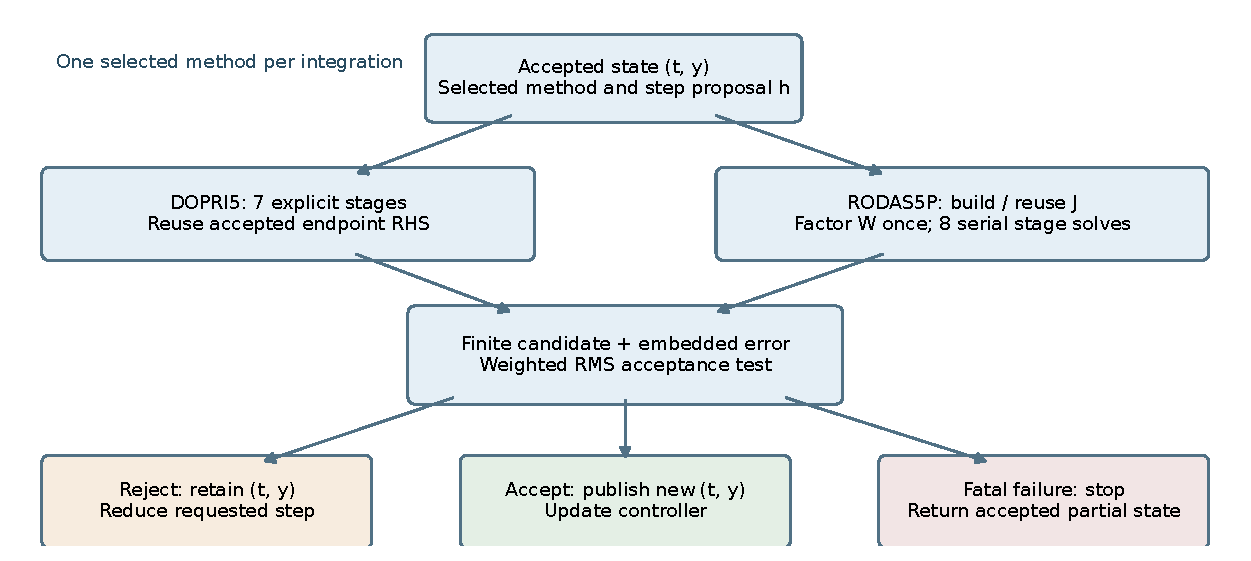
\includegraphics{figures/accepted_state_flow.pdf}
\caption{수락 상태를 중심으로 한 시간 적분. 한 실행에서 선택한 방법의
단계 계산을 수행한 뒤 오차를 검사한다. 거절과 수치 실패는 확정 상태를
덮어쓰지 않는다.}
\end{figure}

\hypertarget{uxba85uxc2dcuxc801-uxc801uxbd84-uxc138uxc158}{%
\subsection{명시적 적분
세션}\label{uxba85uxc2dcuxc801-uxc801uxbd84-uxc138uxc158}}

\texttt{Dopri5::with\_session}은 전체 시간 구간과 관측 일정을 먼저
정의하고, closure 안에서 제한된 시도 횟수만큼 진행할 수 있는 세션을
제공한다. 세션은 \texttt{advance\_to}를 통해 진행하고, 수락 상태를
가리키는 체크포인트를 조회한다. 일시 중지는 새 적분을 반복해서 시작하는
것과 다르다. 저장된 첫 우변, 제어기 정보, 전체 시도 예산을 보존한다.

\textbf{명제 7.} 같은 초기 상태, 동일한 전체 관측 일정, 같은 유효성
식별값을 사용하는 결정적 우변에 대해, 시도 경계에서의 일시 중지가 상태를
변경하지 않는다면 세션 실행은 중단 없는 실행과 같은 수락 궤적을 갖는다.

\textbf{증명.} 초기 상태와 내부 작업공간이 같다고 하자. 다음 시도의 우변
입력, 저장된 첫 도함수, 요청 간격 및 남은 예산이 같으면 단계 계산과 수락
판단도 같다. 일시 중지는 이 값을 바꾸지 않으므로 수락 여부와 갱신된
상태가 일치한다. 시도 횟수에 대한 귀납법을 적용한다. \(\square\)

이 명제는 사전에 동일한 관측 일정이 주어진 경우에 한정된다. 중간에
새로운 관측 경계를 삽입하거나, 우변의 숨은 상태를 바꾸거나, 모델
매개변수를 갱신한 실행이 원래 궤적과 같다는 뜻은 아니다. 세션의 유효성
식별값은 모델과 설정의 변경을 식별하기 위한 계약이다. 식별값이 바뀐
호출은 우변을 실행하지 않고 오류를 반환하며, 변경된 모델에는 새 세션을
구성해야 한다. closure가 반환되면 세션도 종료되어 바깥에서 재개할 수
없다. 정상 완료 전에 반환한 결과는 부분해이며 성공 여부는
\texttt{false}이다. 수락 끝점에서 멈추는 사용자 판단도 연속 사건 함수의
근을 찾는 기능과 구별한다.

\hypertarget{uxacc4uxc0b0uxb7c9uxacfc-uxba54uxbaa8uxb9ac}{%
\section{계산량과
메모리}\label{uxacc4uxc0b0uxb7c9uxacfc-uxba54uxbaa8uxb9ac}}

\(C_f\)를 한 우변 평가 비용, \(C_J\)를 한 Jacobian 구성 비용, \(b\)를
고정 대역폭 규모, \(m\)을 선형 반복 풀이에서 저장하는 기저 크기로 쓰자.
아래 비용은 한 시도에 대한 점근적 연산량이며, 벽시계 시간의 보장이
아니다.

\begin{longtable}[]{@{}
  >{\raggedright\arraybackslash}p{(\columnwidth - 4\tabcolsep) * \real{0.3333}}
  >{\raggedright\arraybackslash}p{(\columnwidth - 4\tabcolsep) * \real{0.3333}}
  >{\raggedright\arraybackslash}p{(\columnwidth - 4\tabcolsep) * \real{0.3333}}@{}}
\toprule\noalign{}
\begin{minipage}[b]{\linewidth}\raggedright
방법과 구조
\end{minipage} & \begin{minipage}[b]{\linewidth}\raggedright
주요 비용
\end{minipage} & \begin{minipage}[b]{\linewidth}\raggedright
작업공간
\end{minipage} \\
\midrule\noalign{}
\endhead
\bottomrule\noalign{}
\endlastfoot
DOPRI5 & 최초 \(7C_f\), 정상 연속 시도 \(6C_f\) 및 \(O(n)\) 벡터 연산 &
\(O(n)\) \\
조밀 RODAS5P & \(C_J+8C_f+O(n^3)+8O(n^2)\) & \(O(n^2)\) \\
고정 폭 대역 RODAS5P & \(C_J+8C_f+O(nb^2)+8O(nb)\) & \(O(nb)\) \\
제공 JVP를 쓰는 선형 반복 풀이 & 반복 수에 따른 JVP 및 직교화 비용 &
기저 저장 \(O(nm)\) \\
\end{longtable}

RODAS5P의 \(8C_f\)는 단계의 우변 비용이다. Jacobian을 유한차분으로
만들거나 비자율 시간 편미분을 차분하면 그 평가가 별도로 더해진다. 거절
후 같은 시작 상태에서 재시도할 때는 유효한 Jacobian, 시작 우변 및 시간
편미분을 재사용할 수 있다. 다만 간격 \(h\)가 바뀌므로 \(W_n\)의 분해는
다시 필요하다.

대역의 복잡도는 대역 저장을 실제로 사용하는 경로에 대한 것이다. 조밀
배열에 우연히 0이 많다는 이유만으로 모든 경로의 저장량이 \(O(nb)\)가
되는 것은 아니다. 또한 선형 반복법의 반복 횟수는 차원만으로 정해지지
않는다. 연산자의 스펙트럼, 비정규성 및 조건수에 따라 달라진다. 본 선택
경로가 쓰는 GMRES에는 전처리기가 없으므로, 대규모 또는 조건이 나쁜
문제의 비용을 소수 반복으로 가정할 수 없다.

고정된 정렬 관측 일정의 길이를 \(M\)이라 하면, 세션은 이진 탐색으로 각
진행 목표의 등록 여부를 확인한다. 한 번의 확인은 \(O(\log M)\) 비교를
요구하고, 모든 관측점에 대한 진행 호출을 합하면 이 부분의 비용은
\(O(M\log M)\)이다. 매번 처음부터 일정을 찾는 \(O(M^2)\) 방식과 달리
추가 저장 공간을 요구하지 않는다. 이는 목표 검증에 대한 복잡도이며 우변
평가나 출력 저장의 비용을 줄였다는 주장은 아니다.

적분 작업공간의 재사용은 단계별 임시 벡터 할당을 줄인다. 그러나 전체
공개 함수가 어떤 입력에서도 힙 할당을 전혀 하지 않는다는 사양은 아니다.
입력 검증, 우변이 내부적으로 수행하는 작업, 유한차분 Jacobian의 구성,
출력 표본 저장 및 세션 종료 시의 결과 소유권 이동에는 별도 비용이 생길
수 있다. 보관하는 표본 수가 \(M\)이면 출력 상태 저장 자체에 \(O(Mn)\)가
필요하다.

\hypertarget{uxc0acuxc6a9uxc790uxac00-uxc9c0uxcf1cuxc57c-uxd560-uxc218uxd559uxc801-uxacc4uxc57d}{%
\section{사용자가 지켜야 할 수학적
계약}\label{uxc0acuxc6a9uxc790uxac00-uxc9c0uxcf1cuxc57c-uxd560-uxc218uxd559uxc801-uxacc4uxc57d}}

다음 조건은 계산 결과를 해석하는 데 직접 필요하다.

\begin{enumerate}
\def\labelenumi{\arabic{enumi}.}
\tightlist
\item
  우변은 모든 출력 성분을 유한한 값으로 작성한다. 재시도 중 모델을
  바꾸지 않는다.
\item
  \texttt{Nonstiff}와 \texttt{Stiff} 선언은 문제에 대한 사전 정보이다.
  모르는 경우에는 \texttt{Unknown}을 사용하고, 완료 여부와 작업량을
  확인한다.
\item
  대역, 자율성, Jacobian 및 JVP의 선언은 실제 우변과 일치해야 한다.
  우변만 정확하고 도함수 정보가 틀린 구성도 잘못된 문제 정의이다.
\item
  절대 허용오차는 상태 성분의 척도를 반영한다. 국소 RMS와 개별 성분의
  전역 오차를 구별한다.
\item
  시간 정의역의 경계에서 수치 시간 편미분이 허용되는지 확인한다.
  필요하면 \(f_t\)를 제공한다.
\item
  반환된 수치 상태의 성공 여부를 확인한다. 시도 예산 소진 또는 콜백 실패
  뒤의 부분해를 완료된 적분으로 사용하지 않는다.
\item
  장시간 진동과 민감한 파생 관측량에서는 해당 관측량의 수렴을 확인한다.
  안정한 계산과 충분히 정확한 계산은 서로 다른 성질이다.
\end{enumerate}

이 설계는 비강성 문제에서 불필요한 선형 대수를 생략하고, 강성 문제에서는
공유 선형 연산자를 통해 한 단계의 비용을 통제한다. 두 경우에 동일하게
중요한 것은 수치 방법의 이름보다 실제로 허용한 연산, 사용한 오차 척도,
출력의 의미 및 실패 이후 상태의 해석을 명확하게 유지하는 것이다.

\hypertarget{uxcc38uxace0uxbb38uxd5cc}{%
\section{참고문헌}\label{uxcc38uxace0uxbb38uxd5cc}}

{[}1{]} Dormand, J. R. and Prince, P. J. (1980). A family of embedded
Runge-Kutta formulae. \emph{Journal of Computational and Applied
Mathematics}, \textbf{6}(1), 19--26. DOI:
\href{https://doi.org/10.1016/0771-050X(80)90013-3}{10.1016/0771-050X(80)90013-3}.

{[}2{]} Steinebach, G. (2023). Construction of Rosenbrock--Wanner method
Rodas5P and numerical benchmarks within the Julia Differential Equations
package. \emph{BIT Numerical Mathematics}, \textbf{63}, Article 27. DOI:
\href{https://doi.org/10.1007/s10543-023-00967-x}{10.1007/s10543-023-00967-x}.

{[}3{]} Shampine, L. F. (1986). Some practical Runge-Kutta formulas.
\emph{Mathematics of Computation}, \textbf{46}(173), 135--150. DOI:
\href{https://doi.org/10.1090/S0025-5718-1986-0815836-3}{10.1090/S0025-5718-1986-0815836-3}.

\hypertarget{uxbd80uxb85d-uxacc4uxc218uxc640-uxad6cuxd604uxc758-uxb300uxc751}{%
\section{부록: 계수와 구현의
대응}\label{uxbd80uxb85d-uxacc4uxc218uxc640-uxad6cuxd604uxc758-uxb300uxc751}}

계수와 단계식의 재현에는 다음 파일을 사용한다. 이 목록은 수학적 사양과
실제 실행 코드를 대조하기 위한 것이다.

\begin{longtable}[]{@{}
  >{\raggedright\arraybackslash}p{(\columnwidth - 2\tabcolsep) * \real{0.5000}}
  >{\raggedright\arraybackslash}p{(\columnwidth - 2\tabcolsep) * \real{0.5000}}@{}}
\toprule\noalign{}
\begin{minipage}[b]{\linewidth}\raggedright
내용
\end{minipage} & \begin{minipage}[b]{\linewidth}\raggedright
저장소 경로
\end{minipage} \\
\midrule\noalign{}
\endhead
\bottomrule\noalign{}
\endlastfoot
DOPRI5 단계와 유리수 계수 &
\texttt{crates/rodas5p-integrators/src/dopri5.rs} \\
DOPRI5 연속 확장 계수 \(P\) &
\texttt{crates/rodas5p-integrators/src/dopri5\_dense.rs} \\
RODAS5P의 \(\gamma,A,C,c,b^{\rm u},H\) &
\texttt{fixtures/rodas5p\_coefficients\_snapshot.json} \\
\(\Gamma\), \(\alpha\), 출력 계수 변환 &
\texttt{crates/rodas5p-core/src/coefficients.rs} \\
변환된 RODAS5P 단계 계산 &
\texttt{crates/rodas5p-integrators/src/rodas5p\_fast.rs} \\
유한차분 Jacobian & \texttt{crates/vigilode/src/fd.rs} \\
적응형 제어 & \texttt{crates/rodas5p-integrators/src/adaptive.rs} \\
일반 방법 선택 & \texttt{crates/vigilode/src/selection.rs} \\
명시적 세션 & \texttt{crates/vigilode/src/session.rs} \\
\end{longtable}

RODAS5P 계수 파일은 8행 8열의 \(A,C\), 여덟 개의 시간 절점 및 출력
가중치, 3행 8열의 연속 출력 계수 \(H\)를 포함한다. 계수의 현재 배정밀도
표현을 넘어서는 고정밀 정확값이 있다고 가정하지 않는다. 표의 경로와 함께
읽을 수 있도록 별도 기계 가독형 사양에는 단계 수, 오차 차수, 기본값 및
지원 범위를 기록한다.

\end{document}
